\newpage
\section{Analyse des Ausgangszustands und Ableitung des Kriterienkatalogs}
\label{sec:bedrohungsmodell}

Der Maßstab für das zu konstruierende Artefakt stammt aus zwei Quellen der Fallstudie, dem Konzept, mit dem die
Scripting-Engine heute betrieben wird, und dem produktiven Skriptbestand. Aus beiden ergeben sich die
Angriffswege und aus diesen der Kriterienkatalog.

\subsection{Ausgangszustand und Vertrauensannahmen}
\label{sec:systemkontext}

Die Scripting-Engine führt JavaScript auf Node.js aus und verarbeitet damit Webhooks
(\autoref{sec:einleitung:motivation}). Den Code hinterlegt der Mandant selbst. Er wird versioniert gespeichert und
über viele Ausführungen hinweg unverändert wiederverwendet. Die Fähigkeit als Werkzeug eines KI-Agenten besteht im
Produkt noch nicht. Sie gehört deshalb nicht zum Ausgangszustand, sondern ist eine Anforderung an das Artefakt,
das beide Profile tragen muss. Betriebsdaten liegen für das Agentenprofil nicht vor, weshalb alle Aussagen dazu
aus dem Interaktionsmuster eines Agenten hergeleitet und als Annahme gekennzeichnet sind.

Zwei Ressourcen teilen sich die Ausführungen heute, und an beiden muss eine Mandantengrenze
verlaufen. Die erste ist der Host-Kernel. Der Execution Service schaltet seinen Runner-Pods
dafür eine gVisor-Runtime-Klasse vor und ergänzt sie um einen gehärteten Sicherheitskontext, bei
dem Privilege Escalation unterbunden ist, sämtliche Capabilities entzogen sind, das
seccomp-Standardprofil greift und kein Service-Account-Token eingebunden wird. Der rohe Zugriff auf die Systemaufrufe des
Hosts, den generische Containerisierung offenlegt \autocite[S.~17--18]{souppaya_application_2017}, wird
dadurch verkleinert, aber nicht beseitigt.

Welches Skript eine Instanz ausführt, entscheidet sich erst beim Aufruf. Das Skript wird je
Ausführung über eine vorsignierte \ac{URL} aus einem Objektspeicher nachgeladen, weshalb eine Instanz
nicht an ein Skript gebunden ist, sondern nacheinander beliebige Skripte ihres Mandanten
ausführt. Sein Eintrag im Module Cache wird dabei vor jeder Ausführung verworfen, sodass
auch das Übersetzen bei jeder Ausführung erneut anfällt.

Die zweite geteilte Ressource liegt innerhalb dieser Sandbox. Jeder Mandant erhält einen eigenen
Execution Service, sodass Instanzen mandantenübergreifend nicht wiederverwendet werden. Der
Skriptcode wird unmittelbar in den laufenden Node.js-Prozess geladen, ohne einen eigenen
Unterprozess je Ausführung, und es ist höchstens eine Ausführung zur Zeit vorgesehen. Bricht ein
Client eine Anfrage ab, gilt sie für Knative als beendet, und weitere Anfragen erreichen den Pod,
obwohl die Ausführung noch läuft. Aufeinanderfolgende
Ausführungen desselben Mandanten teilen sich damit den Prozessspeicher. Das temporäre Verzeichnis
wird vor jeder Ausführung zurückgesetzt, Heap und globale Variablen bleiben bestehen. Ein
Node.js-Prozess je Mandant statt je Ausführung ist der Ausgangspunkt, gegen den sich jedes
geprüfte Modell messen lassen muss.

Aus diesem Konzept folgen die Schutzziele. \emph{Vertraulichkeit} und \emph{Integrität}
verlangen die Mandantenisolation aus \autoref{sec:grundlagen:eigenschaften}, die \emph{Verfügbarkeit}, dass eine
Ausführung die Bedienung anderer Mandanten nicht beeinträchtigt. Hinzu tritt die \emph{Zustandsfreiheit}, die verlangt, dass eine Ausführung
keinen Zustand an eine spätere weitergibt.

Das vierte Ziel verdient eine genauere Betrachtung, weil sein Charakter am Lastprofil hängt. In
der Webhook-Verarbeitung stammen alle Skripte eines Mandanten von ihm selbst und bilden eine
gemeinsame Vertrauensdomäne. Übernommener Zustand stört dort die folgenden Ausführungen,
überschreitet aber keine Vertrauensgrenze, weshalb Zustandsfreiheit hier eine Anforderung an die
Zuverlässigkeit ist. Im Agentenprofil gilt das nicht mehr. Zwei aufeinanderfolgende Ausführungen
desselben Mandanten entstehen aus verschiedenen Kontexten und können nach V2 von verschiedenen
Dritten beeinflusst sein, sind einander also nicht wechselseitig vertrauenswürdig. Der
Zustandsübertrag wird damit auch innerhalb eines Mandanten zur Vertraulichkeitsverletzung. Die
Vertrauenseinheit verschiebt sich vom Mandanten auf die einzelne Ausführung, und die
Isolationsgrenze muss dieser Verschiebung folgen. Diese Verschiebung ist der Kern des Problems,
das die vorliegende Arbeit löst.

Damit lassen sich die Vertrauensannahmen festhalten.

\begin{description}
  \item[V1: Der ausgeführte Code ist nicht vertrauenswürdig.] Im Webhook-Profil hinterlegt der
    Mandant den Code selbst, kennt ihn und verantwortet ihn. Aus Sicht der Plattform bleibt er
    fremder Code, weil ein Mandant nach V4 bösartig sein kann. Im Agentenprofil entfällt
    zusätzlich die Annahme, der Mandant kenne den Code, denn dieser entsteht erst zur Laufzeit
    und wird vor seinem einzigen Lauf von keinem Menschen gelesen
    \autocite[S.~50208]{wang_executable_2024}. Er gilt in beiden Fällen nicht als fehlerhaft, sondern als
    potenziell aktiv bösartig.

  \item[V2: Im Agentenprofil ist der Code über seine Eingaben von Dritten beeinflussbar.] Das
    Modell erzeugt den Code aus einem Kontext, der Inhalte anderer Personen enthält, und solche
    Inhalte lassen sich gezielt so gestalten, dass sie das Verhalten des Modells steuern
    \autocite[S.~79--80]{greshake_not_2023}. Der Urheber des schädlichen Codes muss deshalb nicht der
    Mandant sein. Dass von Agenten erzeugter Code risikobehaftete Operationen enthalten kann, ist
    empirisch belegt \autocite[S.~106191]{guo_redcode_2024}.

  \item[V3: Die Plattform ist vertrauenswürdig.] Host-Kernel, gVisor, Container-Orchestrierung,
    Laufzeitbinärdatei und Execution Service gelten als korrekt und nicht kompromittiert.
    Angriffe, die diese Bestandteile auf anderem Weg unterwandern, etwa über die
    Kubernetes-Steuerungsebene, liegen außerhalb der Betrachtung. Das codeerzeugende Modell
    gehört nach V5 nicht dazu.

  \item[V4: Die Mandanten misstrauen einander.] Es besteht keine Annahme, dass ein Mandant die
    Ausführungen eines anderen nicht angreift.

  \item[V5: Das codeerzeugende Modell liegt außerhalb der Kontrolle der Plattform.] Der Mandant
    kann ein eigenes Modell anbinden und kontrolliert dann Gewichte, System prompt und
    vorgelagerte Prüfungen vollständig. Aussagen über das Alignment dieses Modells, über seine
    Widerstandsfähigkeit gegen die in V2 beschriebene Beeinflussung oder über die Einhaltung
    einer vorgegebenen Schnittstelle sind deshalb nicht möglich.
\end{description}

V5 hat eine unmittelbare Folge für den Entwurf. Eine Beschränkung der Fähigkeiten, die einem
Skript zur Verfügung stehen, kann nicht über System prompt oder Tool Schema erfolgen, weil beides
dem Mandanten gehört. Sie muss von der Ausführungsumgebung durchgesetzt werden \autocite[S.~1]{ji_taming_2026}. Für das
Agentenprofil verbleibt der Plattform damit keine Schutzmaßnahme außerhalb der Isolationsgrenze.
Die jüngere Forschung zur Sicherheit agentischer Systeme betrachtet diese Frage bislang
überwiegend aus der Perspektive des Modells und weniger aus der der Systemisolation
\autocite[S.~1]{christodorescu_systems_2025}.

\subsection{Struktur des produktiven Skriptbestands}
\label{sec:bestandsanalyse}

Ein Ausführungsmodell, das den heutigen Skripten die benötigte Schnittstelle entzieht, ist
unabhängig von seinen Isolationseigenschaften nicht einführbar. Dieser Abschnitt erhebt deshalb,
welchen Teil der Node.js-Schnittstelle der Bestand tatsächlich braucht.

\subsubsection{Datengrundlage und Vorgehen}

Ausgewertet wurden 1.718 Mandanten mit 14.575 Skriptversionen, die sich auf 8.310 inhaltlich verschiedene Skripte und
4.768 Importe verteilen. Vollständig minifizierte Inhalte sind ausgeschlossen, weil sich ihre Importe statisch nicht
zuverlässig bestimmen lassen (269 Inhalte, 519 Skriptversionen, 25 Mandanten), eine Gegenrechnung ohne den Filter
verschiebt die Kennzahlen um gut einen Prozentpunkt. Jedes Skript wird anhand seiner Importe klassifiziert, wobei die
härteste Einschränkung zählt, und ein Mandant erhält die Einstufung seines härtesten Skripts. Die Analyse ist
statisch und sieht weder dynamisch zusammengesetzte Modulnamen noch gebündeltes Kompilat, 24 Skripte fallen als
Parse-Fehler an und gelten vorsorglich als blockierend. Ein Import sagt nichts darüber, was ein npm-Paket seinerseits
benötigt, weshalb für die Pakete mit nennenswertem Mandantengewicht der ausgelieferte Quelltext gelesen wurde, 27 von
203 verwendeten Paketen, die 87,9\,\% der npm-nutzenden Mandanten erreichen.

\subsubsection{Ergebnis}

713 Mandanten (41,5\,\%) benötigen eine Schnittstelle, die eine sprachbasierte Laufzeit ohne
vermitteltes Binding nicht bereitstellt. Diese Gruppe wird im Folgenden als Hard Floor
bezeichnet. Werden die Mandanten, deren Pakete vollständig außerhalb der geprüften Menge liegen,
pessimistisch als nicht lauffähig gewertet, ergibt sich ein Viabilitätsintervall von 39,0\,\% bis
42,9\,\%.

\begin{figure}[H]
  \centering
  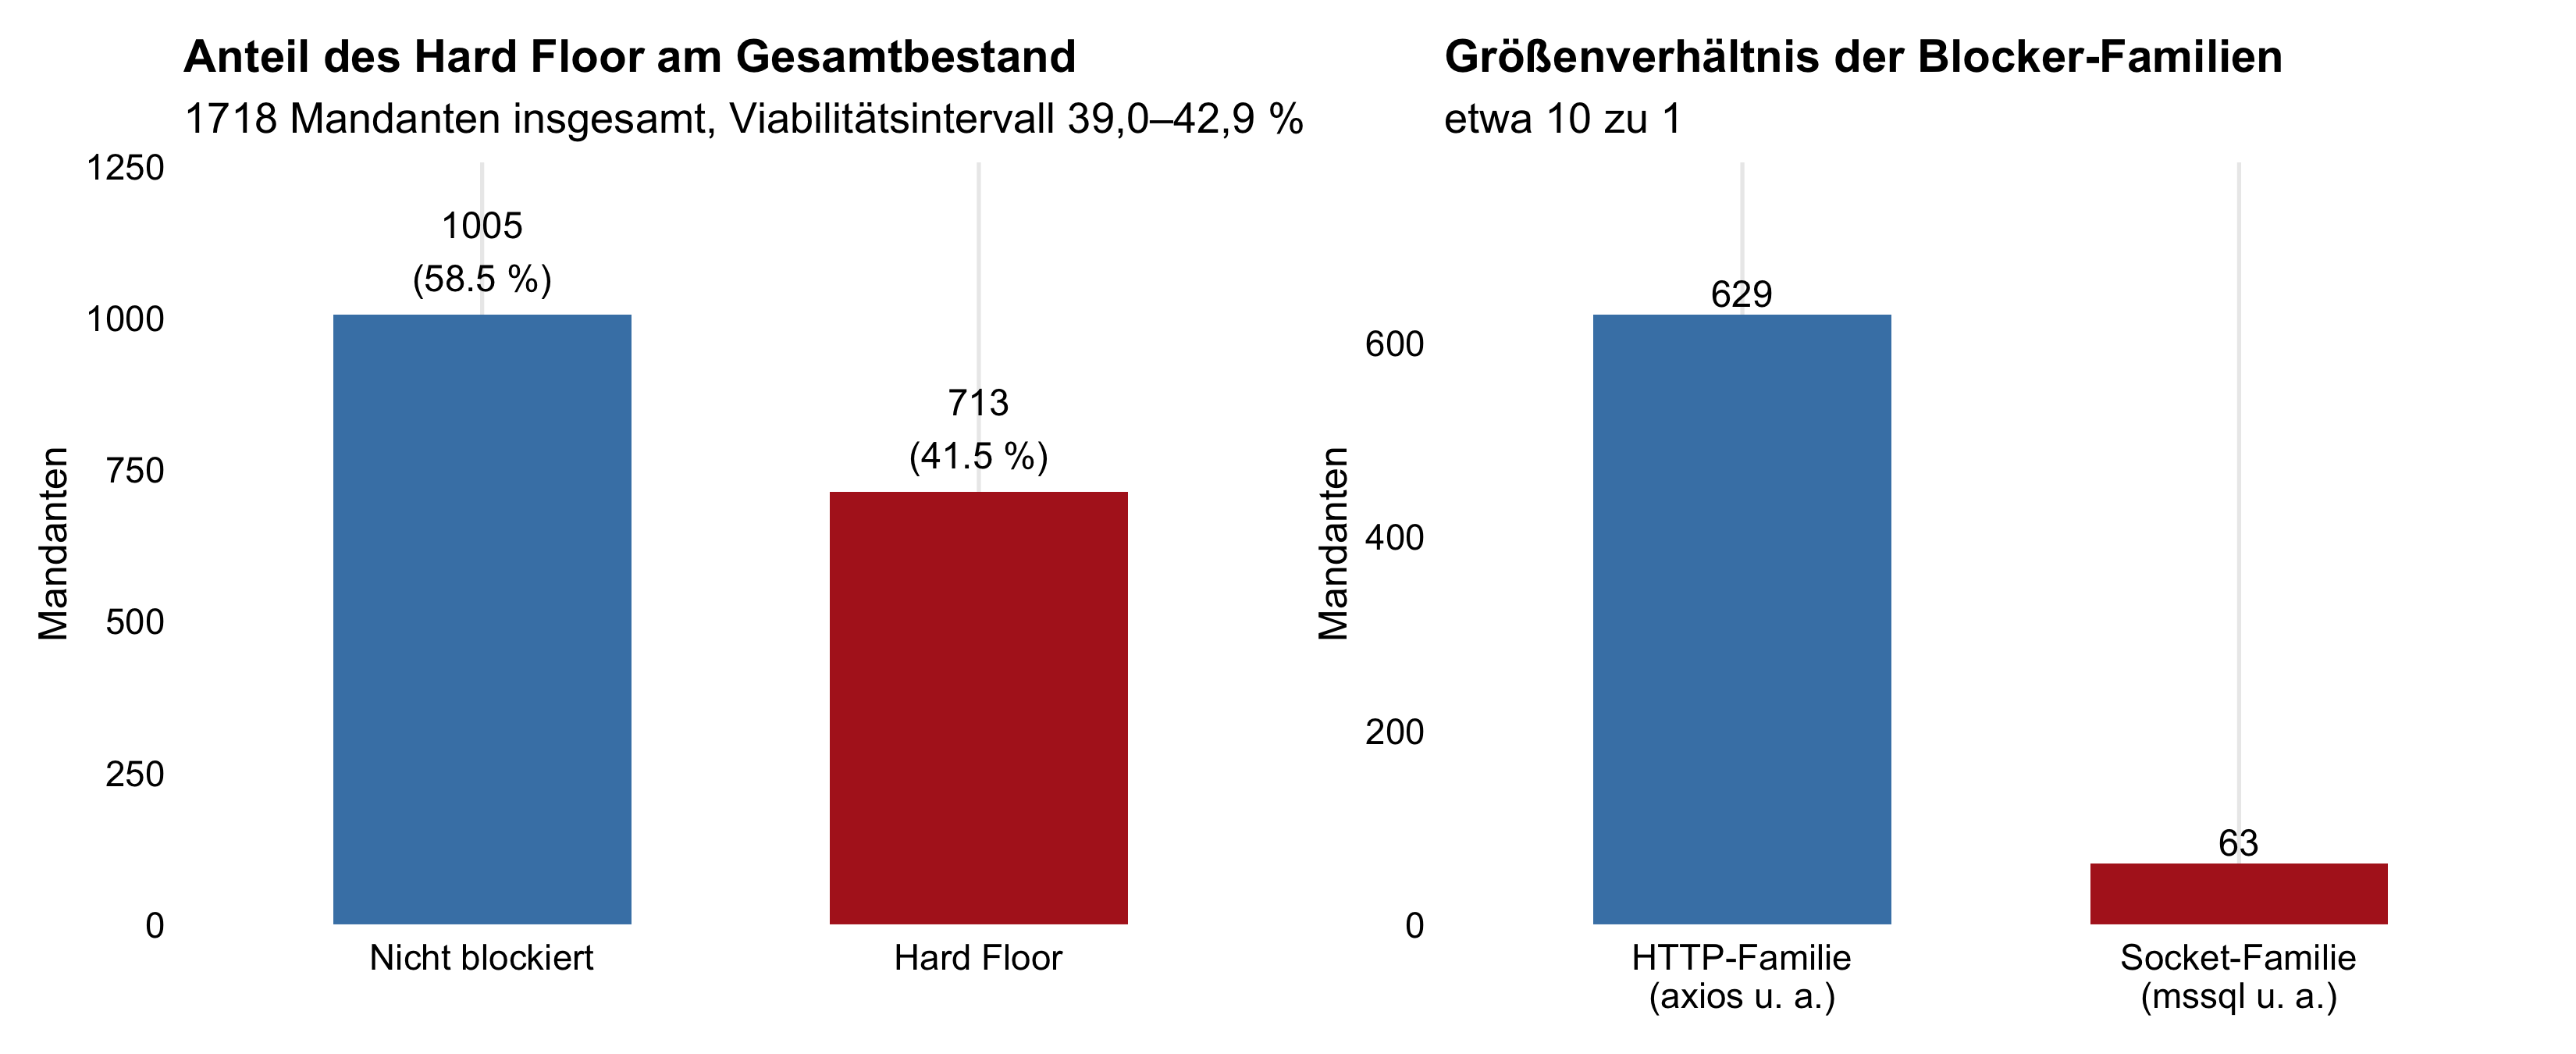
\includegraphics[width=\textwidth]{hard_floor_einordnung.png}
  \caption{Anteil des Hard Floor am Gesamtbestand und Größenverhältnis der beiden
    blockierenden Paketgruppen}
  \label{fig:hard-floor-einordnung}
\end{figure}

Die blockierenden Pakete zerfallen in zwei Gruppen mit deutlich verschiedenem Bedarf. Die eine benötigt \ac{HTTP}
direkt und umgeht ein bereitgestelltes \texttt{fetch}, 14 Pakete bei 629 Mandanten, am häufigsten \texttt{axios} mit
579. Die andere benötigt einen rohen \ac{TCP}- oder \ac{TLS}-Socket, 8 Pakete bei 63 Mandanten, am häufigsten
\texttt{mssql} mit 46. 44 Mandanten gehören zu beiden Gruppen, die Vereinigung umfasst 648 der 713 blockierten
Mandanten, also 90,9\,\%, die an einem Netzwerk-Binding und an nichts anderem scheitern. Die übrigen 65 brauchen
Dateisystem, Betriebssystemmodule oder Prozesse. Die Kompatibilitätsschranke ist damit eng umrissen, und zwischen
den beiden Gruppen liegt ein Größenunterschied von etwa zehn zu eins.

Die kleinere Gruppe stellt die schwierigere Anforderung. Ihre Vertreter sind überwiegend
Datenbanktreiber mit eigenem binären Protokoll. Bei \texttt{mssql} und dem darunterliegenden
\texttt{tedious} wird die Verbindung im Klartext aufgebaut und erst danach auf \ac{TLS}
umgestellt. Ein bereitgestelltes \texttt{fetch} hilft dieser Gruppe nicht.

Neben den Paketen erfasst die Auswertung, welche Node-Globals ein Skript ohne Import erreicht,
etwa \texttt{Buffer} oder \texttt{process.env}. Nach dem jeweils härtesten Merkmal eingeteilt,
kommen 81,9\,\% der 8.310 verschiedenen Skripte ohne jede Node-spezifische \ac{API} aus und
50,9\,\% ohne jeden Import, und 15,6\,\% nutzen ein Node-Global und 2,1\,\% ein Node-Kernmodul. Die
Abhängigkeit von Node-Globals konzentriert sich auf zwei Namen: \texttt{process.env} bei 519
Mandanten (30,2\,\%) und \texttt{Buffer} bei 396 Mandanten (23,1\,\%). Danach fällt die Verbreitung
um eine Größenordnung, \texttt{\_\_dirname} erreicht noch 20 Mandanten, jedes weitere Mitglied von
\texttt{process} unter zehn. Beide häufigen Namen lassen sich in einer eingebetteten Engine
nachbilden, ohne eine Umgebungsautorität freizugeben. Sie bestimmen den Umfang der
Kompatibilitätsschicht in \autoref{sec:kompatibilitaetsschicht}, nicht ihre Machbarkeit. Die
Erkennung ist eine Analyse freier Bezeichner und zählt einen Namen nur, wenn das Skript ihn
nirgends selbst bindet. Sie untertreibt daher eher, als dass sie Abhängigkeiten erfindet.

Ein zweiter Befund betrifft die Größe der gebündelten Artefakte. Von den 14.575 Skriptversionen binden 2.373 npm-Pakete
ein, und das fertige Bundle liegt im Median bei 69,3\,KB, im 95.\ Perzentil bei 429,0\,KB und im Maximum bei 1,41\,MB,
typischerweise den Faktor zehn bis dreißig über dem Quelltext. Betroffen sind 1.023 der 1.718 Mandanten, je Mandant
liegt die Zahl gebündelter Versionen im Median bei zwei, im 95.\ Perzentil bei dreizehn, im Einzelfall bei 151. Für
die Kompatibilität ist das ohne Belang, für den Entwurf nicht, weil das Bundle nach \autoref{sec:zustellung} bei jeder
Ausführung zugestellt und ausgewertet werden muss und ohne Cache der Abruf bei jeder Ausführung auf den Anfragepfad
fällt.

\subsubsection{Grenzen der Auswertung}

Der Datensatz deckt allein die heutige Webhook-Verarbeitung ab, zum Agentenprofil, das im Produkt nichts zu migrieren
hat, lässt sich aus ihm nichts ableiten. Aufrufzahlen enthält er nicht, ein Mandant mit einem Skript pro Monat wiegt so
schwer wie einer mit hoher Aufruffrequenz, weshalb die Mandantenquote eine Obergrenze der praktischen Betroffenheit
ist und keine Schätzung. Die transitive Hülle ist unvollständig, was das angegebene Intervall abbildet. Die Auswertung
erfolgte aggregiert, ohne Codeausschnitte und ohne Mandantenkennungen.

\subsection{Angreifermodell und relevante Angriffswege}
\label{sec:angreifermodell}

Das Angreifermodell wird über Fähigkeiten bestimmt und nicht über Identität. Die maßgebliche
Fähigkeit besteht darin, beliebigen JavaScript-Code innerhalb der Ausführungsumgebung eines
Mandanten auszuführen. Sie ist durch die Bauart des Dienstes gegeben und muss nicht erst erlangt
werden. Die Codeausführung ist damit kein Angriffsziel, sondern der Ausgangspunkt, und die
maßgebliche Frage lautet, was der Code von dort aus erreichen kann. Dieselbe Ausgangslage
kennzeichnet die Bewertung von Ausbruchsfähigkeiten aktueller Sprachmodelle, bei der der Zugang
innerhalb des Containers vorausgesetzt und allein der Ausbruch untersucht wird
\autocite[S.~3]{marchand_quantifying_2026}.

Wer den Code verfasst, ist für diese Fähigkeit unerheblich. Nach V1 kann es ein bösartiger Mandant
sein, nach V2 im Agentenprofil auch ein Dritter, dessen Inhalte in den Kontext des Modells
gelangen. Beide Urheber führen auf dieselbe technische Lage. Die Ziele des Angreifers entsprechen
den negierten Schutzzielen aus \autoref{sec:systemkontext}. Alles, was V3 der Plattform zurechnet,
gehört nicht zu seinen Fähigkeiten, also weder physischer Zugriff noch ein Zugang auf dem Host
außerhalb der Ausführungsumgebung noch eine Netzwerkposition im Plattforminneren.

Die verbleibenden Angriffswege lassen sich nach der Schicht ordnen, auf der die ausgenutzte
Ressource geteilt wird, entsprechend der Einordnung von Angriffswegen serverloser Plattformen
nach Anwendungs- und Infrastrukturebene \autocite[S.~8]{marin_serverless_2022}.

\subsubsection{A1, Anwendungsebene: Zustand zwischen Ausführungen}

Weil der Code in denselben Prozess geladen wird, überdauern über \texttt{setTimeout} oder \texttt{setInterval}
registrierte Callbacks das Ende ihrer Ausführung und können Daten späterer Ausführungen mitlesen
\autocite{dvelop_ag_dvelop_2026}. Ebenso überdauern globale Variablen, veränderte Prototypen und offene Verbindungen,
denn das Zurücksetzen des Dateisystems und das Verwerfen des Module Cache greifen nur für Zustand auf Datei- und
Modulebene. Da eine Instanz genau einen Mandanten bedient, verläuft dieser Weg innerhalb eines Mandanten, und seine
Bewertung folgt der Verschiebung der Vertrauenseinheit aus \autoref{sec:systemkontext}. Derselbe geteilte Prozess trägt
einen zweiten Weg: Eine Ausführung kann Ressourcen so erschöpfen, dass die Instanz für folgende Ausführungen
unbrauchbar wird, wie ein Vorfall im Ausgangszustand belegt, bei dem ein Verfügbarkeitstest im Minutentakt eine Instanz
dauerhaft aktiv hielt und ein Speicherleck ihren Verbrauch bis zur Unbrauchbarkeit steigen ließ.

\subsubsection{A2, Sprachebene: geteilte Laufzeit im selben Prozess}

% GRUNDLAGEN: Mikroarchitekturelle Seitenkanaele und Spectre gehoeren als Begriff
% nach Kapitel 2. Hier bleibt nur die Folgerung fuer das Bedrohungsmodell.

Der zweite Weg greift eine Isolationsgrenze an, die innerhalb eines Prozesses verläuft und
Angriffe unterhalb der Softwareebene nicht abfangen kann. Über einen entfernten Timer ließ sich
aus einem ko-lokierten Cloudflare Worker ein \ac{JWT} mit bis zu zwölf Bit pro Sekunde bei
einer Genauigkeit von rund 99 Prozent auslesen, und zwar auf einer produktiven Plattform, die V8
Isolates einsetzt \autocites[S.~1]{schwarzl_remote-timer-as--service_2026}{schwarzl_revisit_2026}. Denselben Befund hatte zuvor
die Einführung der Site Isolation in Chrome, wo eine sprachbasierte Trennung zweier Origins im
gemeinsamen Prozess nach Bekanntwerden von Spectre \autocite[S.~1]{kocher_spectre_2019} nicht mehr trug und durch eine Prozessgrenze
ersetzt wurde \autocites[S.~1661--1662]{reis_site_2019}[S.~1]{mcilroy_spectre_2019}. Cloudflare benennt die daraus folgenden Restrisiken für
V8 Isolates ausdrücklich \autocite{cloudflare_security_2026}. Eine sprachbasierte Grenze allein
bildet damit keine hinreichende Mandantengrenze.

\subsubsection{A3, Infrastrukturebene: Sandbox-Laufzeit und Host-Kernel}

Der dritte Weg zielt auf den Ausbruch aus der Ausführungsumgebung. Generische Containerisierung
trägt diese Grenze nur eingeschränkt. Das \ac{NIST} führt den geteilten Kernel als eigene
Angriffsfläche und hält fest, dass ein Container eine Sandbox nicht vollwertig ersetzt
\autocite[S.~7, 18]{souppaya_application_2017}. Eine Untersuchung an neun öffentlichen Ausbruchs-Exploits
zeigt, dass eine Einschränkung der Containerrechte über User Namespaces sieben davon abwehrt,
zwei aber erfolgreich bleiben \autocite[S.~44]{reeves_towards_2021}. Die Fallstudie begegnet dem bereits
über gVisor (\autoref{sec:grundlagen:isolation}). Die Angriffsfläche verschwindet dadurch nicht,
sie verlagert sich auf den Sentry, der selbst in Software implementiert und angreifbar ist, was
eine gezielte Fuzzing-Untersuchung belegt \autocite[S.~168]{li_g-fuzz_2024}.

Der Weg bleibt damit relevant, wenn auch auf höherem Niveau. Ein Agent mit Codeausführung im Container kann
Fehlkonfigurationen, Kernel-Schwachstellen sowie Schwächen der Laufzeit und der Orchestrierung selbst auffinden und
ausnutzen \autocite[S.~1]{marchand_quantifying_2026}, auch wenn die Untersuchung Container ohne vorgeschaltete
Sandbox-Laufzeit betrifft. Sie beschreibt den Angreifertyp, dem die Grenze standhalten muss: Aus einem menschlichen
Angreifer mit vorbereitetem Exploit wird der ausgeführte Workload selbst.

\subsection{Kriterienkatalog}
\label{sec:kriterienkatalog}

Der Katalog übersetzt die Ergebnisse der vorangegangenen Abschnitte in einen Maßstab. Jedes Kriterium ist auf einen
Angriffsweg, eine Vertrauensannahme, die Bestandsanalyse oder eine Betriebsanforderung zurückführbar, Kriterien ohne
solche Herkunft werden nicht aufgenommen. \emph{Muss-Kriterien} beschreiben Eigenschaften, ohne die ein
Ausführungsmodell ausscheidet, sie werden einzeln geprüft, nicht verrechnet und entscheiden die Vorauswahl in
\autoref{sec:vorauswahl}. \emph{Soll-Kriterien} beschreiben graduelle Unterschiede, scheiden nichts aus und bilden den
gewichteten Maßstab, an dem \autoref{sec:Evaluation} das Artefakt gegen den Ausgangszustand bewertet. Die Trennung ist
Voraussetzung dafür, dass das Artefakt scheitern kann, denn ein Modell mit gutem Nutzwert, das ein Muss-Kriterium
verletzt, ist keine Lösung.

\subsubsection{Muss-Kriterien}

\begin{table}[H]
  \caption{Muss-Kriterien, Herkunft und Nachweis}
  \label{tab:musskriterien}
  \small
  \begin{tabularx}{\textwidth}{@{}l >{\RaggedRight\arraybackslash}X >{\RaggedRight\arraybackslash}p{0.18\textwidth} >{\RaggedRight\arraybackslash}p{0.18\textwidth}@{}}
    \hline
    Nr. & Kriterium & Herkunft & Nachweis \\
    \hline
    M1 & \textbf{Prozessgrenze je Mandant.} Zwischen zwei Mandanten verläuft eine Grenze auf
         Prozess- oder Virtualisierungsebene. Eine sprachbasierte Grenze allein genügt nicht. &
         A2 & Architektur\-prüfung \\[2pt]
    M2 & \textbf{Zustandsfreiheit je Ausführung.} Kein Zustand einer Ausführung ist einer
         späteren zugänglich, auch nicht innerhalb eines Mandanten. Umfasst Prozessspeicher,
         globale Variablen, registrierte Callbacks, offene Verbindungen und Dateisystem. &
         A1, Verschiebung der Vertrauens\-einheit & Prüffälle T1 bis T6 \\[2pt]
    M3 & \textbf{Keine größere Kernel-Oberfläche.} Die dem Gastcode zugängliche Oberfläche des
         Host-Kernels wächst gegenüber dem Ausgangszustand nicht. &
         A3 & Konfigurations\-vergleich \\[2pt]
    M4 & \textbf{Vermittelter Zugriff.} Netz und Dateisystem ausschließlich über Bindings, die
         die Ausführungsumgebung vermittelt. Keine Beschränkung beruht auf Mitwirkung des
         Modells. & V5 & Prüffälle T7 bis T9 \\[2pt]
    M5 & \textbf{Verfügbarkeit bei Knotenupdates.} Die Zeit ohne Ausführungsfähigkeit während
         eines rollierenden Knotenupdates überschreitet den festgelegten Wert nicht. &
         Betriebs\-anforderung, vier Updates je Jahr & Messung gegen den Ausgangszustand \\
    \hline
  \end{tabularx}
\end{table}

M2 ist auf aufeinanderfolgende Ausführungen geschnitten, weil der Ausgangszustand je Prozess eine Ausführung
vorsieht. Gleichzeitige Ausführungen entstehen dort nur über abgebrochene Anfragen, im Modell durch mehrere Slots je
Pod (\autoref{sec:betriebsplanung}). M3 ist gegen den Ausgangszustand formuliert, weil dieser mit gVisor bereits einen
User-Space-Kernel einsetzt, ein Modell, das diese Schicht aufgibt, wäre auf der Infrastrukturebene ein Rückschritt,
auch bei besserem Nutzwert. M4 folgt aus V5, denn die Schnittstelle zur Ausführungsumgebung ist der einzige
Durchsetzungspunkt, den die Plattform kontrolliert, und entspricht dem Prinzip der Complete Mediation
\autocite[S.~1282]{saltzer_protection_1975}. Der Zielwert von M5 ist relativ: Die Zeit ohne
Ausführungsfähigkeit darf die des Ausgangszustands im selben Versuch nicht überschreiten, und keine begonnene
Ausführung darf verloren gehen, eine absolute Schranke wäre aus der Betriebsanforderung nicht herleitbar.

\subsubsection{Soll-Kriterien und Gewichtung}

\begin{table}[H]
  \caption{Soll-Kriterien, Messgrößen und Gewichte, absteigend nach Gewicht}
  \label{tab:sollkriterien}
  \small
  \begin{tabularx}{\textwidth}{@{}l >{\RaggedRight\arraybackslash}p{0.23\textwidth} >{\RaggedRight\arraybackslash}X r@{}}
    \hline
    Nr. & Kriterium & Messgröße & Gewicht \\
    \hline
    S1 & Kaltstartlatenz & Zeit bis zum Ausführungsbeginn beim ersten Auftrag eines Mandanten, P95,
         S1a mit Pod aus dem Pool, S1b bei leerem Pool & 0,30 \\
    S6 & Kompatibilität des Bestands & Anteil unverändert lauffähiger Mandanten und
         Skripte & 0,25 \\
    S2 & Warme Latenz & Ausführungslatenz bei warmer Instanz, P50 bis P99 & 0,15 \\
    S3 & Speicherbedarf & Bedarf je Pod unter Last und je Mandant im Ruhezustand & 0,10 \\
    S7 & Aufwand für den Rest & Aufwand, den nicht lauffähigen Anteil zu überführen & 0,10 \\
    S4 & Durchsatz & Ausführungen je Sekunde bei gesättigter Last & 0,10 \\
    \hline
    \multicolumn{3}{@{}l}{Summe} & 1,00 \\
    \hline
  \end{tabularx}
\end{table}

Die Gewichte sind eine begründete Setzung und kein Messergebnis. S1 erhält das höchste Gewicht,
weil die Kaltstartzeit im Agentenprofil in die Wartezeit der anfragenden Person eingeht und sich
über die Aufrufe einer Aufgabe summiert \autocite[S.~76]{dean_tail_2013}. S6 folgt darauf, weil \autoref{sec:bestandsanalyse} die
Kompatibilität als stärkste Gegenkraft zu einem Wechsel des Ausführungsmodells ausweist. Die
übrigen Kriterien wiegen leichter, weil sie entweder die Ausführung selbst betreffen, ohne die
Wartezeit im gleichen Maß zu prägen wie S1, oder weil sie Restgrößen abdecken, deren Größenordnung
bereits durch S6 begrenzt ist. Die Bewertung je Kriterium erfolgt auf einer Skala von null bis
fünf, und der Nutzwert ist die mit den Gewichten gebildete Summe. Maßgeblich ist bei Kriterien mit
Vergleichswert der Faktor, um den der Prototyp besser ist: null Punkte beim Faktor null,
drei bei gleichem Wert, fünf ab dem Faktor zwei, dazwischen jeweils linear, sodass ein Wert knapp unter
dem des Ausgangszustands knapp unter drei Punkte erhält. Gerundet wird erst das Ergebnis je
Kriterium auf ganze Punkte. S1 geht je zur Hälfte aus S1a und S1b ein, bei S1 zählt das 95.\ Perzentil, bei S2 der Median. S6 und S7 erhalten je angefangene zwanzig Prozent der
Mandanten, die unverändert laufen beziehungsweise keine Anpassung brauchen, einen Punkt. Die
Zuordnung der Messwerte zu den Punkten legt \autoref{sec:Evaluation} offen, damit die Bewertung
nicht von der Darstellung abhängt.

Der Zielwert ist für S1 und S2 der Wert des Ausgangszustands im selben Messaufbau, den der Prototyp unterbieten muss.
Eine Zahl wird nicht vorab gesetzt, weil der Ausgangszustand bisher nicht unter den Lastprofilen dieser Arbeit
gemessen wurde. S3 und S4 werden dem Ausgangszustand gegenübergestellt, ohne dass ein Zielwert sie entscheidet. S6 und
S7 haben keinen Vergleichswert, ihr Maßstab ist die Bestandsanalyse aus \autoref{sec:bestandsanalyse}.

\subsubsection{Prüffallkatalog}

M2 und M4 lassen sich nicht durch Architekturbetrachtung allein belegen. Für sie gilt ein Katalog von Prüffällen
(\autoref{tab:prueffaelle} im Anhang), abgeleitet aus den Angriffswegen A1 bis A3 und gegen den Ausgangszustand und
das Artefakt ausgeführt, sodass die Gegenüberstellung zugleich belegt, welche Eigenschaften der Ausgangszustand bereits
erfüllt. T1 und T6 bilden dokumentierte Vorgänge des Ausgangszustands nach, T4 prüft, ob dessen Reset des temporären
Verzeichnisses auch im Artefakt greift, und die übrigen Fälle ergänzen Wege aus derselben geteilten Ressource, die
noch nicht beobachtet wurden. Einen vergleichbaren Katalog für Umgebungen, die nicht vertrauenswürdigen, von
Sprachmodellen erzeugten Code ausführen, enthält SandboxEval mit 51 Eigenschaften
\autocite[S.~1--2]{rabin_sandboxeval_2025}, zugeschnitten auf Python und Linux und in
\autoref{sec:pruefung-isolation} für JavaScript angepasst ergänzend ausgeführt.

